\section{Introduction}
\label{sec:introduction}

\vspace{-0.2cm}

\begin{wrapfigure}{R}{0.5\linewidth}
	\vspace{-2.0cm}
	\begin{center}
		\includegraphics[width=0.9\linewidth]{figures/3d_sparsity}
	\end{center}
	\vspace{-0.5cm}
	\caption{The sparsity characteristic of 3D data in occupancy grid representation. 3D occupancy grids in resolution $30$, $64$ and $128$ are shown in this figure, together with their density, defined as $\frac{\#occupied~grid}{\#total~grid}$. It is clear that 3D occupancy grid space gets sparser and sparser as the fidelity of the surface approximation increases.}
	\label{fig:3d_sparsity}
	\vspace{-0.3cm}
\end{wrapfigure}

Rapid advances in 3D sensing technology have made 3D data ubiquitous and easily accessible, rendering them an important data source for high level semantic understanding in a variety of environments. The semantic understanding problem, however, remains very challenging for 3D data as it is hard to find an effective scheme for converting input data into informative features for further processing by machine learning algorithms. For semantic understanding problems in 2D images, deep CNNs~\cite{Lecun_IEEE98_Gradient} have been widely used and have achieved great success, where the convolutional layers play an essential role. They provide a set of 2D filters, which when convolved with input data, transform the data to informative features for higher level inference.
%The pattern of the 2D filters defines a feature extraction scheme. An important reason for the success of CNNs is that the feature extraction scheme --- the 2D filter patterns --- is adapted to the training data as opposed to being hand-crafted. In this manner they can outperform most carefully hand-crafted features.

In this paper, we focus on the problem of learning a 3D shape representation by a deep neural network. We keep two goals in mind when designing the network: the shape features should be \emph{discriminative} for shape recognition and \emph{efficient} for extraction at runtime. However, existing 3D CNN pipelines that simply replace the conventional 2D filters by 3D ones~\cite{WU_CVPR15_3D,Maturana_IROS15_VoxNet}, have difficulty in capturing geometric structures with sufficient efficiency. The input to these 3D CNNs are voxelized shapes represented by occupancy grids, in direct analogy to pixel array representation for images. We observe that the computational cost of 3D convolution is quite high, since convolving 3D voxels has cubical complexity with respect to spatial resolution, one order higher than the 2D case. Due to this high computational cost, researchers typically choose $30 \times 30 \times 30$ resolution to voxelize shapes~\cite{WU_CVPR15_3D,Maturana_IROS15_VoxNet}, which is significantly lower than the widely adopted resolution $227\times 227$ for processing images~\cite{Russakovsky_IJCV15_ImageNet}. We suspect that the strong artifacts introduced at this level of quantization (see Figure~\ref{fig:3d_sparsity}) hinder the process of learning effective 3D convolutional filters.

\begin{figure}[t!]
	\vspace{-0.5cm}
	\begin{center}
		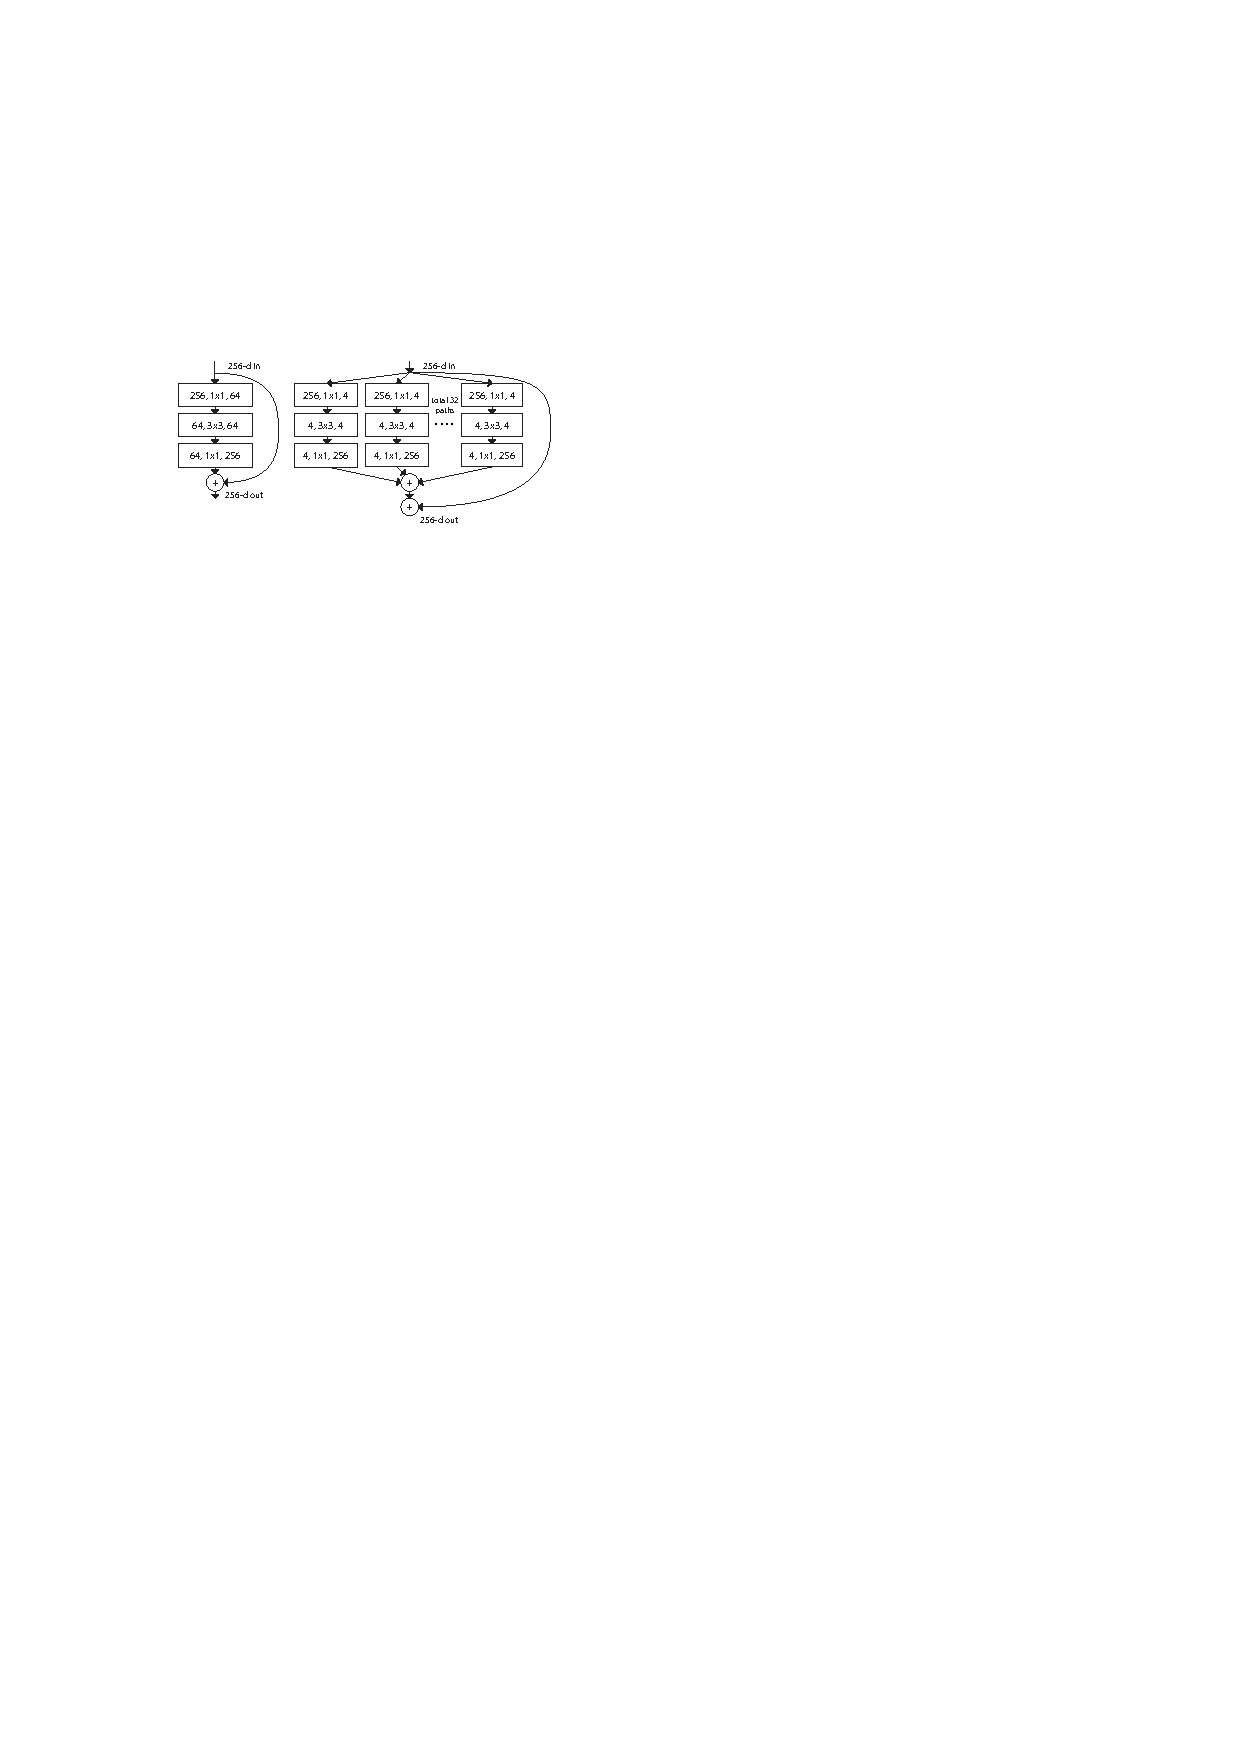
\includegraphics[width=0.9\linewidth]{figures/teaser}
	\end{center}
	\vspace{-0.3cm}
	\caption{An visualization of probing filters before (a) and after (d) training them for extracting 3D features. The colors associated with each probing point visualize the filter weights for them. Note that probing points belong to the same filter are linked together for visualizing purpose. (b) and (c) are subsets of probing filters of (a) and (d), for better visualizing that not only the weights on the probing points, but also their locations are optimized for them to better ``sense'' the space.}
	\label{fig:teaser}
	\vspace{-0.6cm}
\end{figure}

Two significant differences between 2D images and 3D shapes interfere with the success of directly applying 2D CNNs on 3D data. First, \emph{as the voxel resolution grows, the grids occupied by shape surfaces get sparser and sparser} (see Figure~\ref{fig:3d_sparsity}). The convolutional layers that are designed for 2D images thereby waste much computation resource in such a setting, since they convolve with 3D blocks that are largely empty and a large portion of multiplications are with zeros. Moreover, \emph{as the voxel resolution grows, the local 3D blocks become less and less discriminative}. To capture informative features, long range connections have to be established for taking distant voxels into consideration. This long range effect demands larger 3D filters, which yields an even higher computation overhead.

To address these issues, we represent 3D data as 3D fields, and propose a \emph{field probing} scheme, which samples the input field by a set of {\em probing filters} (see Figure~\ref{fig:teaser}). Each probing filter is composed of a set of probing points which determine the shape and location of the filter, and filter weights associated with probing points. In typical CNNs, only the filter weights are trained, while the filter shape themselves are fixed. In our framework, due to the usage of 3D field representation, both the weights and probing point locations are trainable, making the filters highly flexible in coupling long range effects and adapting to the sparsity of 3D data when it comes to feature extraction. The computation amount of our field probing scheme is determined by how many probing filters we place in the 3D space, and how many probing points are sampled per filter. Thus, the computational complexity does not grow as a function of the input resolution. We found that a small set of field probing filters is enough for sampling sufficient information, probably due to the sparsity characteristic of 3D data.

Intuitively, we can think our field probing scheme as a set of sensors placed in the space to collect informative signals for high level semantic tasks. With the long range connections between the sensors, global overview of the underlying object can be easily established for effective inference. Moreover, the sensors are ``smart'' in the sense that they learn how to sense the space (by optimizing the filter weights), as well as where to sense (by optimizing the probing point locations). Note that the intelligence of the sensors is not hand-crafted, but solely derived from data. We evaluate our field probing based neural networks (FPNN) on a classification task on ModelNet~\cite{WU_CVPR15_3D} dataset, and show that they match the performance of 3DCNNs while requiring much less computation, as they are designed and trained to respect the sparsity of 3D data.
